\documentclass[tikz,border=10pt]{standalone}
\usepackage{amsmath}
\begin{document}
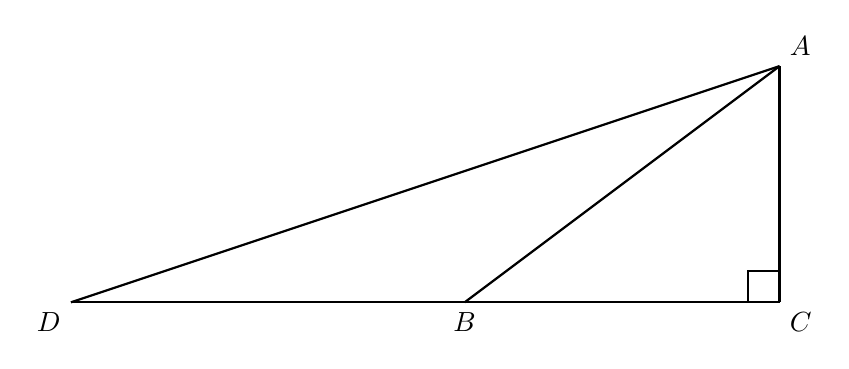
\begin{tikzpicture}[thick, scale=1]
  % Points
  \coordinate (D) at (0,0);
  \coordinate (B) at (5,0);
  \coordinate (C) at (9,0);
  \coordinate (A) at (9,3);

  % Edges (all solid)
  \draw (D) -- (A);
  \draw (A) -- (B);
  \draw (D) -- (C);
  \draw (A) -- (C);

  % Right-angle mark at C
  \draw (8.6,0) -- (8.6,0.4) -- (9,0.4);

  % Labels
  \node[below left] at (D) {$D$};
  \node[below] at (B) {$B$};
  \node[below right] at (C) {$C$};
  \node[above right] at (A) {$A$};
\end{tikzpicture}
\end{document}
